\documentclass[11pt]{article}

%!TEX root = ../main/main.tex

\usepackage[utf8]{inputenc}
\usepackage{fullpage}
\usepackage{epsfig}
\usepackage{amsmath}
\usepackage{amssymb}
\usepackage{multicol}
\usepackage{color}
\usepackage{hyperref}
\usepackage{xcolor}
\usepackage{dirtree}
\usepackage{fontawesome}
\usepackage{tikz}
\usepackage{../packages/pythonhighlight}
\usepackage{../packages/logo}

\usetikzlibrary{trees}

%!TEX root = ../main/main.tex

\newcommand{\comm}[1]{{\bf {\color{red} #1}}}
\newcommand{\Enc}{\textit{Enc}}
\newcommand{\Dec}{\textit{Dec}}


\begin{document}

%!TEX root = ../main/main.tex

\begin{tabular}{ccl}
\begin{tabular}{c}

\psfig{file=../images/puclogo.eps}
\end{tabular}
&\ \ \ &
\begin{tabular}{l}
PONTIFICIA UNIVERSIDAD CATOLICA DE CHILE\\
ESCUELA DE INGENIERIA\\
DEPARTAMENTO DE CIENCIA DE LA COMPUTACION
\end{tabular}
\end{tabular}

\vspace{.2cm}

\begin{center}
  \bf Criptografía y Seguridad Computacional - IIC3253\\
  \bf Tarea 3\\
  \bf Plazo de entrega: viernes 1 de julio
\end{center}

%!TEX root = ../main/main.tex

\section*{Instrucciones}

Cualquier duda sobre la tarea se deberá hacer en los \emph{issues} del \href{https://github.com/UC-IIC3253/2022}{repositorio del curso}. Si quiere usar alguna librería en sus soluciones debe preguntar primero si dicha librería está permitida. El foro es el canal de comunicación oficial para todas las tareas.

\paragraph{Entrega.} Para entregar esta tarea deberá usar el mismo repositorio que utilizó para entregar las tareas 1 y 2. Al entregar esta tarea, su repositorio se deberá ver exactamente de la siguiente forma:

\bigskip

\dirtree{%
.1 \faGithub \ Repositorio.
.2 \faFolderOpenO \ Tarea 1.
.3 ....
.2 \faFolderOpenO \ Tarea 2.
.3 ....
.2 \faFolderOpenO \ Tarea 3.
.3 \faFolderOpenO \ Pregunta 1.
.4 \faFileTextO \ \texttt{requirements.txt}.
.4 \faFileCodeO \ \texttt{pregunta1.ipynb}.
.2 \faFileTextO \ \texttt{.gitignore}.
.2 \faFileTextO \ \texttt{README.md}.
.2 \faFolderO \ .git.
}

\bigskip

Deberá considerar lo siguiente:

\begin{itemize}

  \item El archivo \texttt{requirements.txt} dentro de la carpeta de una pregunta deberá especificar todas las librerías que se necesitan instalar para ejecutar el código de su respuesta a dicha pregunta. Este archivo debe seguir la especificación de \href{https://pypi.org/project/pip/}{Pip}, es decir se debe poder ejecutar el comando \texttt{pip install -r requirements.txt} suponiendo una versión de \texttt{Pip} mayor o igual a 20.0 que apunta a la versión 3.9 de Python. Si su respuesta no requiere librerías adicionales, este archivo debe estar vacío (pero debe estar en su repositorio).

\item La solución de cada problema de programación debe ser entregada como un Jupyter Notebook (esto es, un archivo con extensión \texttt{ipynb}). Este archivo debe contener comentarios que expliquen claramente el razonamiento tras la solución del problema, idealmente utilizando \emph{markdown}. Más aun, su archivo deberá ser exportable a un módulo de Python utilizando el comando de consola
\begin{verbatim}
    jupyter nbconvert --to python preguntaX.ipynb
\end{verbatim}
Este comando generará un archivo \texttt{preguntaX.py}, del cual se deben poder importar las funciones y clases que se piden en cada pregunta. Por ejemplo, luego de ejecutar este comando, se debe poder importar desde otro archivo Python (ubicado en el mismo directorio) la clase \texttt{EllipticCurve} simplemente con \texttt{from pregunta1 import EllipticCurve}.

%\item Para cada problema cuya solución se deba entregar como un documento (en este caso sólo la Pregunta 1), usted deberá entregar un archivo \texttt{.pdf} que, o bien fue construido utilizando \LaTeX, o bien es el resultado de digitalizar un documento escrito a mano. En caso de optar por esta última opción, queda bajo su responsabilidad la legibilidad del documento. Respuestas que no puedan interpretar de forma razonable los ayudantes y profesores, ya sea por la caligrafía o la calidad de la digitalización, serán evaluadas con la nota mínima.

\end{itemize}


\section*{Preguntas}
Utilizaremos la notación vista en clases, en particular $||$ representa la concatenación.

\begin{enumerate}
    \item 
%!TEX root = ../main/main.tex

En esta pregunta deberá implementar la construcción de Merkle-Damgård
de funciones de hash para mensajes de largo arbitrario, utilizando la
construcción de Davies-Meyer para funciones de
compresión. Concretamente, deberá escribir un Jupyter notebook de
acuerdo a las instrucciones explicadas arriba que contenga las
siguientes funciones:
\begin{python}
def davies_meyer(encrypt: (bytearray, bytearray) -> bytearray,
                 l_key: int, l_message: int) -> (bytearray) -> bytearray:
    """
    Arguments:
      encrypt: an encryption function
      l_key: length in bytes of the keys for encrypt
      l_message: length in bytes of the messages for encrypt
    Returns:
      A compression function from messages of length l_key + l_message to
      messages of length l_message, defined by using the Davies-Meyer
      construction   
    """
\end{python}

\begin{python}
def pad(message: bytearray, l_block: int) -> bytearray:
    """
    Arguments:
      message: message to be padded
      l_block: length in bytes of the block
    Returns:
      extension of message that includes the length of message
      (in bytes) in its last block
    """
\end{python}

\begin{python}
def merkle_damgard(IV: bytearray, comp: (bytearray) -> bytearray,
                   l_block: int) -> (bytearray) -> bytearray:
    """
    Arguments:
      IV: initialization vector for a hash function
      comp: compression function to be used in the Merkle-Damgard
      construction
      l_block: length in bytes of the blocks to be used in the Merkle-Damgard
      construction
    Returns:
      A hash function for messages of arbitrary length, defined by using
      the Merkle-Damgard construction
    """
\end{python}    
Como un ejemplo de cómo pueden ser utilizadas estas funciones
considere el siguiente código, donde \verb+AES_128+ es una función que
implementa el algoritmo de cifrado AES con llaves y mensajes de 16
bytes (128 bits).
\begin{python}
if __name__ == "__main__":
    compresion = davies_meyer(AES_128, 16, 16)
    hash = merkle_damgard(bytearray(b'0123456789012345'), compresion, 16)
    s1 = bytearray(b'Este es un mensaje de prueba para la tarea 2')
    s2 = bytearray(b'Este es un segundo mensaje de prueba para la tarea 2')
    h1 = hash(s1)
    h2 = hash(s2)
    print(h1)
    print(h2)
\end{python}    

\medskip

\paragraph{Corrección.}
Para corregir esta pregunta se utilizará la siguiente implementación de \verb+AES_128+
\begin{python}
from Crypto.Cipher import AES

def AES_128(key: bytearray, message: bytearray) -> bytearray:
    a = AES.new(bytes(key), AES.MODE_ECB)
    return bytearray(a.encrypt(bytes(message)))
\end{python}
y se realizarán los siguientes tests:
\begin{itemize}
\item 4 tests para verificar su implementación de la función \verb+davies_meyer+, cada uno con un puntaje de 0.25,

\item 4 tests para verificar su implementación de la función \verb+pad+, cada uno con un puntaje de 0.5, y

\item 4 tests para verificar su implementación de la función \verb+merkle_damgard+, cada uno con un puntaje de 0.75.
\end{itemize}

\medskip
 \medskip

    \item 
%!TEX root = ../main/main.tex

Considere un esquema criptográfico $(\textit{Gen}, \textit{Enc}, \textit{Dec})$ definido sobre los espacios $\mathcal{M} = \mathcal{K} = \mathcal{C} = \{0,1\}^n$. Suponga además que $\textit{Gen}$ no permite claves cuyo primer bit sea $0$, y que el resto de las claves son elegidas con distribución uniforme. Demuestre que este esquema no es una pseudo-random permutation con una ronda, si $\frac{3}{4}$ es considerada como una probabilidad significativamente mayor a $\frac{1}{2}$.

\medskip

\paragraph{Corrección.}
Esta pregunta se corrige considerando que se debe diseñar una estrategia para el adversario que le permita ganar en una ronda con una probabilidad mayor o igual a $\frac{3}{4}$.
\begin{itemize}
    \item{[3 puntos]} Solo se entrega una estrategia que permite al adversario ganar con una probabilidad mayor o igual a $\frac{3}{4}$.
    
    \item{[4.5 puntos]} Se entrega una estrategia que permite al adversario ganar con una probabilidad mayor o igual a $\frac{3}{4}$, y se formula de manera correcta la probabilidad de que el adversario gane.

    \item{[6 puntos]} Se entrega una estrategia que permite al adversario ganar con una probabilidad mayor o igual a $\frac{3}{4}$, se formula de manera correcta la probabilidad de que el adversario gane, y se muestra que esta probabilidad es mayor o igual a $\frac{3}{4}$.
\end{itemize}

\medskip










\medskip

 \medskip

    \item 
%!TEX root = ../main/main.tex

Un \href{https://en.wikipedia.org/wiki/Merkle_tree}{árbol de Merkle} es una estructura de datos que utiliza una función de hash criptográfica $h$ para representar un conjunto de strings $S=\{s_1,\ldots,s_m\}$. La estructura es un árbol binario en el que cada nodo es un string definido recursivamente: Las hojas son $h(s_1),\ldots,h(s_m)$ y cada nodo interior $n$ se define como $h(n_1 \| n_2)$ donde $n_1$ y $n_2$ son los hijos de $n$ y $\|$ representa la concatenación de strings. Cuando la cantidad de nodos en un nivel es impar se duplica el último nodo de dicho nivel, lo que implica que todos los nodos interiores tienen exactamente dos hijos. La Figura~\ref{fig:merkle} muestra gráficamente la construcción de un árbol de Merkle:

\begin{figure}[h]
  \scriptsize
  \begin{center}
    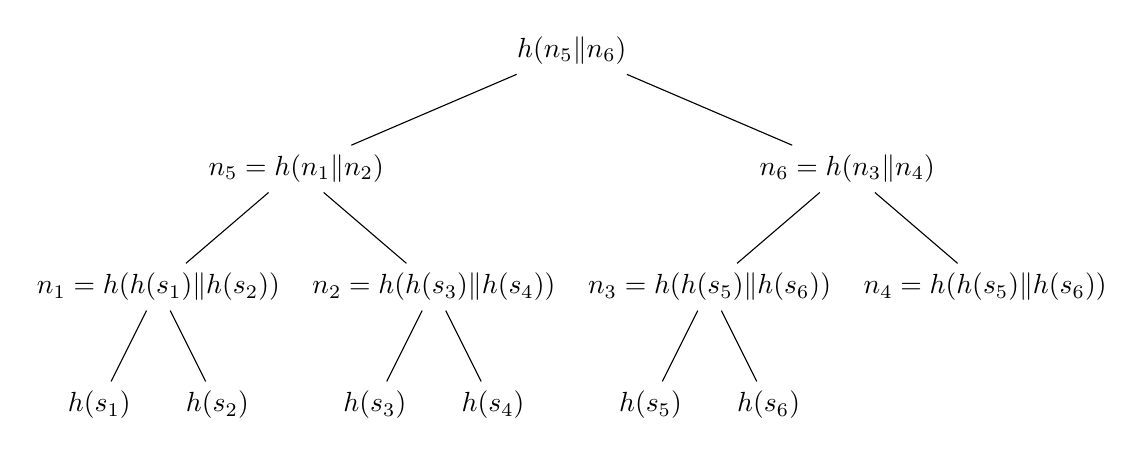
\begin{tikzpicture}[
      level distance=1.5cm,
      level 1/.style={sibling distance=7cm},
      level 2/.style={sibling distance=3.5cm},
      level 3/.style={sibling distance=1.5cm}
    ]
    \node{$h(n_5\|n_6)$}
    child {
      node{$n_5=h(n_1\|n_2)$}
        child {
          node {$n_1=h(h(s_1)\|h(s_2))$}
          child {
            node {$h(s_1)$}
          }
          child {
            node {$h(s_2)$}
          }
        }
        child {
          node {$n_2=h(h(s_3)\|h(s_4))$}
          child {
            node {$h(s_3)$}
          }
          child {
            node {$h(s_4)$}
          }
        }
      }
      child{
        node{$n_6=h(n_3\|n_4)$}
        child{
          node {$n_3=h(h(s_5)\|h(s_6))$}
          child{
            node{$h(s_5)$}
          }
          child{
            node{$h(s_6)$}
          }
        }
        child{
          node {$n_4=h(h(s_5)\|h(s_6))$}
        }
      }

      ;
    \end{tikzpicture}
  \end{center}
  % 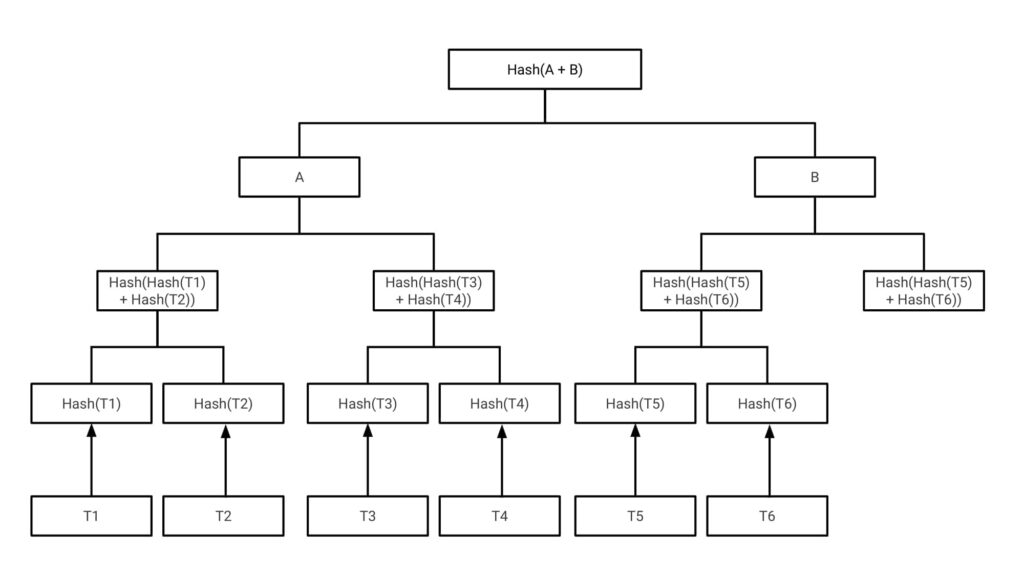
\includegraphics[width=\linewidth]{../images/merkle_tree.jpeg}
  \caption{Árbol de Merkle para el conjunto $S=\{s_1,\ldots,s_6\}$.}
  \label{fig:merkle}
\end{figure}

La principal propiedad de un árbol de Merkle es que si una persona posee un hash que representa la raíz del árbol, la podemos convencer rápidamente de que un elemento es una de las hojas del árbol. Para esto, basta con compartir con esa persona dicho elemento, su hermano y los hermanos de todos sus ancestros, indicando para cada uno si es hermano derecho ($d$) o izquierdo ($i$). Por ejemplo, supongamos que alguien tiene la raíz del árbol que se muestra en la Figura~\ref{fig:merkle}. Para convencer a dicha persona de que $s_5$ es parte del conjunto $S$ basta con enviarle el valor $s_5$ junto con $(h(s_6),d)$, $(n_4,d)$ y $(n_5,i)$. Teniendo estos valores, esta persona puede:

\begin{itemize}
  \item Computar $n_3=h(h(s_5)\|h(s_6))$.
  \item Computar $n_6=h(n_3\|n_4)$.
  \item Computar $h(n_5\|n_6)$ y verificar que el resultado sea igual a la raíz del árbol.
\end{itemize}

En esta pregunta usted deberá programar una clase que permita crear árboles de Merkle para conjuntos arbitrarios de strings, usando una función de hash arbitraria. Deberá seguir las instrucciones indicadas más arriba, entregando un Jupyter Notebook que define una clase como la siguiente:

\bigskip
\begin{python}
  class MerkleTree:
    
    def __init__(self, strings: [str], hash_func: (str) -> str) -> MerkleTree:
    """
    Arguments:
      strings: The set of strings S
    """

    def get_root(self) -> string:
    """
    Returns:
      root: Root of the Merkle Tree
    """

    def get_proof_for(self, item: str) -> None || [(str, "d"|"i")]:
    """
    Returns:
      result: None if the item is not part of the leafs of the tree
              A list with the necessary info to prove that the
              item is part of the leafs of the tree
    """
\end{python}

Además de esta clase, usted deberá programar una función que reciba una \emph{prueba} de que un elemento es parte de un árbol de Merkle, y retorne \texttt{True} si la prueba es correcta y \texttt{False} de lo contrario. Esta función también deberá estar escrita en su Jupyter Notebook y deberá tener la siguiente firma:

\bigskip
\begin{python}
  def verify(root: string, item: str, proof: [(str, "d"|"i")]) -> bool:
    """
    Arguments:
      root: The root of a merkle tree
      item: An abritrary string
      proof: An alleged proof that item is part of a Merkle
             tree with root root
    Returns:
      correct: whether the proof is correct or not
    """
\end{python}


\medskip

\paragraph{Corrección.} Esta pregunta se corrige automáticamente en base a ejemplos, verificando para varios árboles cada funcionalidad. En el archivo con la solución (\texttt{P3.ipynb}) están todos los detalles de la corrección.


\medskip

 \medskip

    \item %!TEX root = ../main/main.tex

Explique la estructura de un par de llaves RSA y la relación entre ellas.

\textbf{Solución:} Un par de llaves RSA se ve como $(e, N)$ y $(d, N)$, y la relación entre estas llaves es que el valor $N$ es la multiplicación de dos números primos $P,Q$ y $e$ es inverso de $d$ en módulo $(P-1)(Q-1)$.

\textbf{Corrección:} Se considerará correcta una respuesta que mencione todos los elementos anteriores y que indique que $e$ es inverso de $d$ en módulo $\phi(N)$.
 \medskip

    \item %!TEX root = ../main/main.tex

Un Message Authentication Code es una función para autentificar mensajes en base a una llave simétrica. Esta función toma una llave $k$ y un mensaje $m$ para generar un tag $t$. Intuitivamente, esperamos que una persona con la llave $k$ pueda verificar que el tag $t$ es válido para el mensaje $m$, y que alguien sin acceso a dicha llave no pueda autentificar mensajes que no se han autentificado antes. Para formalizar esta noción, en clases definimos un \emph{juego} que constaba de cinco pasos.
\begin{enumerate}
  \item El verificador genera una llave $k$ al azar.
  \item El adversario envía un mensaje $m$ al verificador.
  \item $\ldots$
  \item Los pasos 2 y 3 se repiten tantas veces como quiera el adversario.
  \item $\ldots$
\end{enumerate}
Escriba los dos pasos faltantes, y luego explique cuándo decimos que el adversario gana el juego.

\textbf{Solución:} Los pasos faltantes son:
\begin{itemize}
\item[(c)] El verificador responde con el tag $t$ generado con la llave $k$ y el mensaje $m$.
\item[(e)] El adversario envía un mensaje $m_0$ junto a un tag $t_0$, tal que $m_0$ es distinto de todos los mensajes enviados en el paso (b).
\end{itemize}
El adversario gana cuando $t_0$ es un tag válido para el mensaje $m_0$ dada la llave $k$.

\textbf{Corrección:} Se considerará correcta una respuesta que sea equivalente a lo anterior. En particular, la condición de que $m_0$ sea distinto a todos los mensajes enviados anteriormente podría considerarse como parte de lo necesario para que el adversario gane el juego.
 \medskip

    \item %!TEX root = ../main/main.tex

Ciertos documentos son aceptados por instituciones cuando están verificados por un notario y el notario asegura que el documento se puede utilizar en dicha entidad. A modo de ejemplo, la Universidad Católica aceptará una fotocopia de un título profesional siempre que un notario firme un mensaje que diga ``Esta fotocopia de su título es válida, y se puede utilizar en la Universidad Católica''.

Suponga que se quiere digitalizar lo explicado arriba bajo los siguientes supuestos:
\begin{itemize}
  \item Existe un solo notario que tiene una llave secreta y una llave pública.
  \item Todo el mundo conoce la llave pública del notario.
  \item Cada entidad $E$ tiene un string identificador $\text{ID}_E$ conocido por todos. Todos estos identificadores tienen el mismo largo.
\end{itemize}

Ahora, cuando una entidad $E$ pida a un cliente un documento firmado y autorizado por el notario, se usará el siguiente protocolo.

\begin{enumerate}
  \item El cliente genera el documento $d$ y encripta $\text{ID}_E || d$ con la llave pública del notario (suponemos que el documento es también un string). El texto cifrado resultante, que llamaremos $c$, es enviado al notario.
  \item El notario verifica que el documento es válido y se puede utilizar en la entidad correspondiente. De no ser así se termina el protocolo.
  \item El notario genera una firma $f$ para $c$ con su llave privada y le envía $f$ al cliente.
  \item Finalmente, el cliente envía $(c,f)$ a la entidad $E$.
\end{enumerate}

Para tener esta pregunta correcta deberá responder correctamente a las siguientes tres preguntas: (1) ¿Por qué el protocolo no satisface lo esperado? (2) ¿Cómo podemos modificar el último paso para arreglarlo? (3) ¿Qué complejidad innecesaria tiene el protocolo?

\textbf{Solución:}
\begin{itemize}
\item[(1)] Porque la entidad $E$ al recibir $(c, f)$ no puede verificar que esta firma corresponde al documento que se necesita, puesto que $c$ sólo se puede decriptar con la llave secreta del notario.
\item[(2)] Basta con enviar $(d,f)$ en lugar de $(c,f)$. Con esto, la entidad $E$ podría primero encriptar $\text{ID}_E || d$ con la llave pública del notario para obtener $c$, y luego verificar que $f$ es una firma válida para $c$.
\item[(3)] Para el objetivo que se busca no es necesario encriptar el documento. El notario podría directamente firmar $\text{ID}_E || d$.
\end{itemize}

\textbf{Corrección:} Se considerará correcta una solución que tenga una respuesta a la pregunta (1) que indique que $E$ no puede validar el documento porque no puede decriptar $c$. Las respuestas a las otras dos preguntas deben simplemente satisfacer los requerimientos del protocolo, no es necesario que sean equivalentes a lo que se menciona arriba. Obviamente, la respuesta a (2) sólo debe modificar el paso (d).

\end{enumerate}

\end{document}
